\chapter{Bağımsız ve Eşleştirilmiş Örneklem t Testleri; Uygun Testin Seçilmesi}
\label{ch:two-sample}

\begin{prismbox}[PrismLight]{Öğrenme çıktıları}
Bu bölümün sonunda:
\begin{itemize}
  \item bağımsız ve eşleştirilmiş araştırma tasarımlarını gözlem yapısından ayırt edebilecek,
  \item iki bağımsız ortalama için Welch \tstat testini ve güven aralığını hesaplayabilecek,
  \item eşleştirilmiş ölçümleri fark puanlarına dönüştürerek uygun \tstat testini uygulayabilecek,
  \item sonuçları etki büyüklüğü, varsayım kontrolü ve araştırma tasarımıyla birlikte raporlayabileceksiniz.
\end{itemize}
\end{prismbox}

\begin{prerequisitebox}
Tek örneklem \tstat testi, standart hata, serbestlik derecesi, \pval-değeri ve güven
aralığı kavramları bilinmelidir. Ortalama, varyans ve standart sapma
hesapları hatırlanmalıdır.
\end{prerequisitebox}

Tek örneklem testinin karar ve raporlama yapısı Bölüm~\ref{sec:one-sample-t}'de
kurulmuştur. Bu bölüm aynı mantığı bağımsız grup farklarına ve eşleştirilmiş
fark puanlarına genişletir.
\ifimoders\else
Üç veya daha fazla bağımsız grup ortalamasının
tek genel testle karşılaştırılması Bölüm~\ref{ch:anova}'da ele alınır.
\fi

\section{Test seçimini belirleyen temel soru}
\label{sec:t-test-choice}

İki ortalamayı karşılaştırırken ilk soru ``kaç sütun var?'' değil,
``ölçümler hangi birimlere aittir?'' sorusudur. Bir gruptaki katılımcı diğer
grupta yer almıyorsa gruplar bağımsızdır. Aynı kişilerin iki zamanda
ölçülmesi, bireylerin anlamlı çiftler hâlinde eşleştirilmesi veya aynı birimin
iki koşulda gözlenmesi ise eşleştirilmiş bir yapı oluşturur.

Yanlış test seçimi standart hatayı değiştirir. Eşleştirilmiş ölçümleri
bağımsız kabul etmek kişiler arasındaki ortaklığı kaybeder; bağımsız kişileri
yapay biçimde eşleştirmek ise veride bulunmayan bir bağımlılık varsayar.

\begin{table}[H]
\centering
\small
\caption{Üç \tstat testinin araştırma tasarımı bakımından karşılaştırılması.}
\label{tab:t-test-design-choice}
\begin{tabularx}{\textwidth}{@{}>{\raggedright\arraybackslash}p{0.23\textwidth}>{\raggedright\arraybackslash}X>{\raggedright\arraybackslash}X@{}}
\toprule
Test & Analiz birimi & Hedef parametre \\
\midrule
Tek örneklem & Bireysel puan & $\mu-\mu_0$ \\
Bağımsız örneklem & İki ayrı grubun puanları & $\mu_1-\mu_2$ \\
Eşleştirilmiş örneklem & Her çiftin fark puanı & $\mu_D$ \\
\bottomrule
\end{tabularx}
\end{table}

\begin{figure}[H]
\centering
\begin{tikzpicture}[x=0.9cm,y=0.55cm]
  \node[font=\small\bfseries,text=PrismBlue] at (2.1,6.0) {Bağımsız gruplar};
  \node[font=\scriptsize] at (1.2,5.4) {A};
  \node[font=\scriptsize] at (3.0,5.4) {B};
  \foreach \y in {1.2,2.0,2.9,3.8,4.6}
    \fill[PrismBlue] (1.2,\y) circle (2.2pt);
  \foreach \y in {1.0,1.7,2.4,3.3,4.2}
    \draw[PrismSubheadingBlue,thick] (2.92,\y-0.08)--(3.08,\y+0.08)
      (2.92,\y+0.08)--(3.08,\y-0.08);
  \node[font=\tiny,align=center,text=PrismGray] at (2.1,0.35)
    {Farklı bireyler;\\noktalar bağlanmaz};

  \begin{scope}[xshift=6.0cm]
    \node[font=\small\bfseries,text=PrismBlue] at (2.1,6.0) {Eşleştirilmiş ölçümler};
    \node[font=\scriptsize] at (1.1,5.4) {Ön};
    \node[font=\scriptsize] at (3.1,5.4) {Son};
    \foreach \a/\b in {1.0/1.8,1.7/2.0,2.5/3.5,3.2/3.8,4.1/4.5} {
      \draw[PrismGray!70] (1.1,\a)--(3.1,\b);
      \fill[PrismBlue] (1.1,\a) circle (2.1pt);
      \fill[PrismSubheadingBlue] (3.1,\b) circle (2.1pt);
    }
    \node[font=\tiny,align=center,text=PrismGray] at (2.1,0.35)
      {Aynı bireyin ölçümleri\\bir çizgiyle eşleşir};
  \end{scope}
\end{tikzpicture}
\caption{Bağımsız ve eşleştirilmiş veri yapılarının görsel karşılaştırması.}
\label{fig:independent-paired-design}
\end{figure}

Tablo~\ref{tab:t-test-design-choice} yöntemleri analiz birimine göre özetler;
Şekil~\ref{fig:independent-paired-design} ise eşleşmenin yalnız eşit grup
büyüklüğü değil, birimler arasında kurulmuş gerçek bir bağ olduğunu gösterir.

\section{Bağımsız örneklemler için Welch \tstat testi}
\label{sec:welch-test}

İki bağımsız grup için hedef, evren ortalamaları farkı
$\mu_1-\mu_2$'dir. Varyansların eşit olduğu güçlü biçimde savunulamıyorsa
Welch testi güvenli bir varsayılan seçimdir \citep{delacre2017}:
\[
t=\frac{\bar X_1-\bar X_2}
{\sqrt{s_1^2/n_1+s_2^2/n_2}}.
\]
Standart hata
\[
\SE(\bar X_1-\bar X_2)
=\sqrt{\frac{s_1^2}{n_1}+\frac{s_2^2}{n_2}}
\]
ve Welch--Satterthwaite serbestlik derecesi
\[
\nu\approx
\frac{(s_1^2/n_1+s_2^2/n_2)^2}
{(s_1^2/n_1)^2/(n_1-1)+(s_2^2/n_2)^2/(n_2-1)}
\]
ile hesaplanır. Serbestlik derecesinin tam sayı çıkması gerekmez.

Fark için yüzde $100(1-\alpha)$ güven aralığı
\[
(\bar x_1-\bar x_2)
\pm t_{1-\alpha/2,\nu}
\SE(\bar X_1-\bar X_2)
\]
biçimindedir. Farkın yönü analizden önce açıkça tanımlanmalıdır; grup 1 eksi
grup 2 ile grup 2 eksi grup 1 aynı bilimsel sonucu zıt işaretlerle verir.

\section{Eşleştirilmiş örneklem \tstat testi}
\label{sec:paired-test}

Her çift için fark
\[
d_i=x_{i,\text{son}}-x_{i,\text{ön}}
\]
olarak tanımlanır. Eşleştirilmiş \tstat testi, fark puanlarının ortalamasına
uygulanan tek örneklem \tstat testidir:
\[
t=\frac{\bar d}{s_D/\sqrt n},
\qquad \nu=n-1.
\]
Buradaki $n$ tek tek ölçümlerin değil, eksiksiz çiftlerin sayısıdır.
Normallik koşulu iki ayrı ölçüm dağılımından çok fark puanlarının dağılımı
için değerlendirilir.

İki ölçümün standart sapmaları $s_1$, $s_2$ ve aralarındaki korelasyon $r$
ise fark puanlarının varyansı
\[
s_D^2=s_1^2+s_2^2-2rs_1s_2
\]
ilişkisiyle açıklanabilir. Pozitif korelasyon farkların değişkenliğini ve
dolayısıyla standart hatayı azaltabilir. Eşleştirilmiş tasarımın kazancı,
eşleşmenin anlamlı ve ölçümlerin gerçekten aynı birimlere ait olmasına
bağlıdır.

\section{Etki büyüklüğü}
\label{sec:t-effect-size}

Bağımsız gruplarda standartlaştırılmış fark çoğunlukla birleşik standart
sapmaya dayalı Cohen $d$ ile özetlenir:
\[
s_p=\sqrt{\frac{(n_1-1)s_1^2+(n_2-1)s_2^2}{n_1+n_2-2}},
\qquad
d=\frac{\bar x_1-\bar x_2}{s_p}.
\]
Welch testi için çıkarımda eşit varyans varsayılmasa da $s_p$, betimsel bir
standartlaştırma olarak kullanılabilir; kullanılan tanım mutlaka belirtilir.
Küçük örneklemlerde Hedges $g$ düzeltmesi düşünülebilir.
Etki büyüklüğünün tanımı ve belirsizliği açıkça raporlanmalıdır
\citep{lakens2013}.

Eşleştirilmiş tasarımda yaygın ölçülerden biri
\[
d_z=\frac{\bar d}{s_D}
\]
değeridir. $d$ ile $d_z$ aynı paydadan üretilmediği için farklı tasarımların
etki büyüklükleri karşılaştırılırken tanımlar açıkça yazılmalıdır.

\section{Varsayımlar ve tasarım kontrolü}

\begin{itemize}
  \item Gözlemlerin bağımsızlığı veri toplama tasarımından değerlendirilir.
  \item Bağımsız gruplarda her katılımcı yalnız bir gruba katkı vermelidir.
  \item Eşleştirilmiş analizde her satır veya kimlik doğru ölçüm çiftiyle eşleşmelidir.
  \item Küçük örneklemlerde dağılım biçimi ve etkili aykırı değerler grafiklerle incelenmelidir.
  \item Eksik çiftlerin nasıl ele alındığı ve analizde kalan çift sayısı raporlanmalıdır.
  \item Rastgele atama yoksa grup farkı kendiliğinden nedensel etki değildir.
\end{itemize}

\begin{assumptionbox}
Test seçimi veri dosyasındaki sütun sayısına göre değil, gözlemlerin nasıl
ilişkilendiğine göre yapılır. İki sütundaki ölçümler farklı kişilerden
geliyorsa eşleştirilmiş test; tek sütundaki grup kodları aynı kişilerin iki
ölçümünü gösteriyorsa bağımsız test uygun değildir.
\end{assumptionbox}

\begin{mistakebox}
Levene testi anlamlı değilse klasik \tstat testinin, anlamlıysa Welch testinin
otomatik seçilmesi güvenilir bir karar kuralı değildir. Welch yaklaşımı eşit
olmayan varyans ve örneklem hacimlerine karşı daha dayanıklıdır; yöntem seçimi
tek bir ön teste bağlanmamalıdır.
\end{mistakebox}

\section{Çözümlü bağımsız grup örneği}

Birinci grupta $n_1=30$, $\bar x_1=78$, $s_1=8$; ikinci grupta
$n_2=28$, $\bar x_2=72$, $s_2=10$ olsun. Standart hata
\[
SE=\sqrt{\frac{8^2}{30}+\frac{10^2}{28}}\approx2{,}39
\]
ve test istatistiği
\[
t=\frac{78-72}{2{,}39}\approx2{,}51
\]
olur. Yaklaşık $sd=51{,}71$ için çift yönlü $p=0{,}015$ ve ortalama farkının
yüzde 95 güven aralığı $[1{,}21;10{,}79]$ bulunur.

Birleşik standart sapma yaklaşık 9,02 olduğundan Cohen etki büyüklüğü
$d=6/9{,}02\approx0{,}67$'dir. Veriler birinci grubun ortalamasının daha
yüksek olduğuna ilişkin kanıt sunmaktadır; fakat deneysel atama yoksa fark
öğretim yönteminin nedensel etkisi olarak yorumlanamaz.

\section{Çözümlü eşleştirilmiş örnek}

Yirmi öğrencide son test--ön test farkının ortalaması 4,2, standart sapması 5
olsun. Standart hata $5/\sqrt{20}\approx1{,}118$ ve
\[
t=\frac{4{,}2}{1{,}118}\approx3{,}76,
\qquad sd=19
\]
olur. Çift yönlü $p=0{,}001$ ve ortalama değişimin yüzde 95 güven aralığı
$[1{,}86;6{,}54]$'tür. Standartlaştırılmış değişim
\[
d_z=\frac{4{,}2}{5}=0{,}84
\]
olarak bulunur. Kontrol grubu yoksa gözlenen artışın yalnız uygulamadan
kaynaklandığı ileri sürülemez; zaman, test alışkanlığı ve başka olaylar da
değişime katkı verebilir.

\section{Yazılım uygulaması: özet ve gerçek veri üzerinden test}

\begin{softwarebox}
\begin{lstlisting}
from scipy import stats
import numpy as np
import pandas as pd

# Ozet istatistiklerden Welch testi
welch = stats.ttest_ind_from_stats(
    mean1=78, std1=8, nobs1=30,
    mean2=72, std2=10, nobs2=28,
    equal_var=False)

# Eslestirilmis testin fark puanlarindan hesaplanmasi
n, mean_diff, sd_diff = 20, 4.2, 5
t_paired = mean_diff / (sd_diff / np.sqrt(n))
p_paired = 2 * stats.t.sf(abs(t_paired), df=n-1)

# Eslikci paketteki gercek Spector verisi
data = pd.read_csv("companion/data/clean/spector_program.csv")
program = data.loc[data.program_participation == 1,
                   "pre_program_test"]
comparison = data.loc[data.program_participation == 0,
                      "pre_program_test"]
real_welch = stats.ttest_ind(program, comparison,
                             equal_var=False)

print(welch)
print(t_paired, p_paired)
print(real_welch)
\end{lstlisting}
Gerçek veri uygulamasında program grubu için $n=14$ ve ortalama 22,43;
karşılaştırma grubu için $n=18$ ve ortalama 21,56'dır. Welch sonucu yaklaşık
$t=0{,}62$, $p=0{,}537$ verir. İki yönlü testte 0,05 düzeyinde TUCE
ortalamalarının eşitliği reddedilmez; bu, grupların eşdeğerliğini veya
atamanın rastgeleliğini kanıtlamaz. Veri setinin özgün kaynağı için bkz.
\citet{spector1980}.
\end{softwarebox}

\Needspace{8\baselineskip}
\subsection{Spector vakası: hesap ile tasarım kanıtını ayırmak}
\label{sec:spector-tasarim-vakasi}

\textbf{Analiz tanımı.} Gözlem birimi öğrencidir. Yerel dosyadaki 32 kaydın
tamamı kullanılır; iki grup farklı öğrencilerden oluşur, satır sırası bir
eşleşme oluşturmaz. Yanıt TUCE puanı, grup göstergesi PSI katılımıdır.
Hedeflenen karşılaştırma program eksi karşılaştırma grubu ortalama farkıdır;
yöntem iki yönlü Welch testidir. Yerel dosyada bu değişkenlerde eksik değer
yoktur. Bu durum özgün araştırmanın izlem kaybı olmadığını göstermez.

\begin{outputguidebox}
\textbf{Kaynak sınırı.} Greene'in veri açıklaması TUCE'yi ön test olarak
tanımlar; burada incelenen belgelerde ölçümün PSI uygulamasına göre zamanı
kesinleşmemiştir \citep{greeneDiscreteChoice}. Pakette korunan
\texttt{pre\_program\_test} sütun adı bu zamanlamanın kanıtı değildir.
Bu nedenle sonuç, program öncesi denklik veya programın öğrenme üzerindeki
etkisi olarak değil, \emph{TUCE puanlarının gruplar arasında karşılaştırılması}
olarak okunur.

Özgün makalenin araştırma tasarımı açıklaması, daha önceki PSI ve kontrol
gruplarından ara düzey makroekonomi dersini almış 32 öğrenciyi ele alır;
gruplara rastgele atamanın nasıl yapıldığını belirtmez \citep{spector1980}.
Rastgele atamanın doğrulanamaması, yapılmadığının kanıtı değildir. Buradaki
Welch hesabı özgün makalenin modelinin yeniden kurulması değildir.
\end{outputguidebox}

\textbf{Görev ve teslim.} Beş maddelik bir karar kaydı yazın. Her maddede
sayısal bilgi ile tasarım hakkında gerekli belgeyi ayırın; yeni test seçerek
daha küçük bir $p$ değeri aramayın.
\begin{enumerate}[label=\arabic*.]
\item Analiz birimini, kullanılan kayıtları ve fark yönünü belirtin.
Neden eşleştirilmiş test seçilmediğini açıklayın.
\item ``Sütunun adı program öncesi test olduğuna göre zamanlama bellidir''
iddiasını düzeltin. Hangi ek bilgiye ihtiyaç vardır?
\item $p=0{,}537$ sonucunu yorumlayın. ``Gruplar denktir; rastgele atama
başarılıdır'' sonucunun neden elde edilemeyeceğini açıklayın.
\item Aynı 32 öğrencinin başka bir değişkenini analiz etmek yeni bağımsız
kanıt mıdır? Atama ile çalışmaya/izleme dahil olmayı ayırın.
\item Sonucu iki cümleyle raporlayın; ileri sürülemeyecek bir iddia ekleyin.
\end{enumerate}

\textbf{Gerekçeli kontrol yanıtları.}
(1) Birim öğrenci, gruplar 14 ve 18 kişidir; fark program eksi
karşılaştırmadır. Aynı kişilerde iki ölçüm veya belgelenmiş çift yoktur.
(2) Sütun adı yerel bir etikettir; TUCE ölçümü ile PSI başlangıcını gösteren
protokol gerekir. (3) Eşit ortalama hipotezi reddedilmez; eşdeğerlik ve
rastgele atama kanıtlanmaz. Eşdeğerlik sorusu önceden gerekçelendirilmiş bir
fark sınırı gerektirir. (4) Aynı kayıtların yeniden kullanımı bağımsız tekrar
değildir; programa atama ve analizde kalma iki ayrı süreçtir.
(5) Örnek rapor: ``32 kayıtta TUCE ortalamaları program grubunda 22,43,
karşılaştırma grubunda 21,56'dır. Welch testinde $t\approx0{,}62$ ve
$p\approx0{,}537$ bulunmuş; zamanlama ve atama açıklığı sağlanmadığından
sonuç program etkisi veya başlangıç denkliği olarak yorumlanmamıştır.''

\textbf{Değerlendirme ölçütleri (10 puan).} Her madde 2 puandır:
(1) birim ve kapsam 1, fark yönü ve eşleşme gerekçesi 1;
(2) etiket--kanıt ayrımı 1, gerekli zamanlama belgesi 1;
(3) test kararı 1, denklik/atama çıkarımını reddetme 1;
(4) bağımsız tekrar olmadığını belirtme 1, atama--izleme ayrımı 1;
(5) sayısal rapor 1, yorum sınırı 1.
Doğru sayılarla birlikte nedensellik veya denklik iddiası içeren rapor,
son maddenin yorum puanını alamaz; hata diğer doğru bileşenleri silmez.

\begin{outputguidebox}
Çıktıda önce test türünü ve farkın yönünü kontrol edin. Ardından grup veya
eksiksiz çift sayılarını, ortalamaları, standart sapmaları, t değerini,
serbestlik derecesini, \pval-değerini, güven aralığını ve etki büyüklüğünü birlikte
okuyun. Eşit varyans varsayan satır ile Welch satırı birbirine
karıştırılmamalıdır.
\end{outputguidebox}

\section{Tamamlayıcı vaka: bloklu bir tarla deneyi}
\label{sec:v1-colt-park}

\textbf{Soru ve kaynak.} Colt Park deneyinde çiftlik gübresi (FYM) ile
gübresiz kontrolün kuru ot verimleri nasıl karşılaştırılır?
\citet{villagalaviz2023} çalışmasının S1 Data ve S1 File ekleri kullanılır.
Bu, makalenin çok göstergeli analizinin tekrarı değil, tek yanıtlı bir
öğretim uyarlamasıdır. Karşılaştırma ve yanıt bu vaka için belirlenmiştir;
yayımlanmış sonuçlardan habersiz yapılmış bir önkayıt değildir.

\textbf{Atama ve kayıt kapsamı.} Yöntem ekinin 2. sayfasına göre 72
parselin tohum eklenmeyen 24'ü incelenir. Her biri 15 m$^2$ olan
parseller üç blokta yer alır. Her blokta FYM, NPK, NPK+FYM ve gübresiz
kontrol için ikişer parsel bulunur; gübreleme rejimleri blok içinde
rastgele atanmıştır. Veri tablosunun blok--rejim sayımları bu açıklamayla
eşleşir. Burada yalnız FYM ve kontrol seçilerek her bloktan dört,
toplam 12 parsel kullanılır. Diğer rejimler ham dosyadan silinmez.

\begin{researchbox}
\textbf{Ölçüm birimi ve izlenebilirlik.} Yanıt, 2011--2014 ortalama kuru
madde verimidir; yıllar ayrı bağımsız parseller değildir. Excel sözlüğü
alanı m$^2$, yöntem ekinin hesap açıklaması ağırlığı gram olarak belirtir;
burada birim g/m$^2$ olarak korunur. Bu değer 15 m$^2$ parselin toplam
ağırlığı veya 2017'deki besin içeriği ölçümü değildir.

Ek dosyada fiziksel parsel numarası ve yıllık ham ölçümler yoktur.
Üretilen \texttt{source\_row}, Excel'in DATA sayfasındaki satırdır;
saha kimliği değildir. Analize giren 12 kayıtta eksik değer yoktur;
bu kontrol, geçmişte hiç ölçüm kaybı olmadığını kanıtlamaz. Eski Spector
örneğinden farklı olarak blok içi atama burada yöntem ekiyle desteklenir;
ancak özgün saha atama tutanağı yeniden denetlenmiş değildir.
\end{researchbox}

\textbf{Analiz tanımı.} Farkın yönü FYM eksi kontroldür. Her blokta iki
grup ortalaması çıkarılır; üç blok farkına eşit ağırlık verilir:
\[
\widehat{\tau}=\frac{1}{3}\sum_{h=1}^{3}
\bigl(\overline{Y}_{h,\mathrm{FYM}}-\overline{Y}_{h,\mathrm{kontrol}}\bigr).
\]
Her blokta aynı sayıda parsel bulunduğu için bu tahmin, iki grubun genel
ortalamalarının farkına da eşittir. Eşleştirilmiş öğrenci çiftleri gibi
parselleri satır sırasıyla eşleştirmek veya blokları yok saymak gerekmez.

\begin{table}[H]
\centering
\caption{Colt Park: blok ortalamaları ve FYM--kontrol farkı (g/m$^2$)}
\label{tab:v1-colt-park}
\begin{tabular}{@{}lrrr@{}}
\toprule
Blok & Kontrol & FYM & Fark \\
\midrule
ONE & 467,563 & 619,629 & 152,066 \\
TWO & 372,961 & 548,338 & 175,377 \\
THREE & 376,764 & 563,784 & 187,020 \\
\midrule
Eşit ağırlıklı ortalama & 405,763 & 577,250 & 171,488 \\
\bottomrule
\end{tabular}
\end{table}

\textbf{Tasarıma dayalı test.} Keskin sıfır hipotezi, seçilen iki rejimin
ilgili parsellerin hiçbirinin yanıtını değiştirmemesidir. NPK ve NPK+FYM
parsellerinin yerleri sabit tutulduğunda, kalan dört parselin ikisine FYM
etiketi vermenin her blokta $\binom{4}{2}=6$ yolu vardır. Bloklar birlikte
$6^3=216$ eş olasılıklı koşullu atama verir. Bunların tamamında
$\widehat{\tau}$ yeniden hesaplanır. İki yönlü uçluk
$|\widehat{\tau}_{\rm atama}|\geq|\widehat{\tau}_{\rm gözlenen}|$
ile tanımlanır. İki atama bu koşulu sağlar:
\[
p_{\rm tam}=\frac{2}{216}=0{,}009259\ldots
\]
Bu, Monte Carlo benzetimi değildir; tohum gerekmez ve pay/paydaya bir
eklenmez. Test, belgelenen atama düzeninin eş olasılıklı koşullu
dağılımına dayanır; farklı bir atama kuralı için aynı dağılım kullanılamaz.

\textbf{Belirsizliği ayrıca belirtme.} Tam test bir güven aralığı değildir.
Tamamlayıcı olarak üç sabit blok etkisi ve ortak FYM etkisi içeren
$Y_{hi}=\alpha_h+\tau Z_{hi}+\varepsilon_{hi}$ modeli kurulmuştur;
$Z=1$ FYM, $Z=0$ kontroldür. Bağımsız, normal, ortak varyanslı hatalar ve
bloklar arasında ortak eklemeli etki varsayımı altında klasik yüzde 95
$t$ aralığı $[106{,}546;\ 236{,}429]$ g/m$^2$'dir. Standart hata 28,162;
artık serbestlik derecesi $12-4=8$'dir. Bu model aralığı tam
rastgeleleştirme testinin tersinden elde edilmemiştir; varsayımları yalnız
küçük $p$ değeriyle doğrulanmaz. Üç blok ve 12 parselde varsayım
incelemesinin gücü sınırlıdır.

\textbf{Raporlama örneği.} ``FYM ve kontrol için altışar parselin
2011--2014 ortalama kuru madde verimleri karşılaştırılmıştır.
Bloklara eşit ağırlıklı fark 171,488 g/m$^2$; blok içi tam
rastgeleleştirme testinde iki yönlü $p=0{,}009259$ bulunmuştur.
Eklemeli blok modelinin klasik yüzde 95 güven aralığı
$[106{,}546;\ 236{,}429]$ g/m$^2$'dir; bu aralık ek model
varsayımlarına dayanır. Rastgele atama, uygun uygulama ve parseller arası
etkileşimsizlik koşulları altında bu düzen içindeki nedensel karşılaştırmayı
destekler. Sonuç tüm çayırlar için bir gübre reçetesi, biyolojik çeşitlilik
sonucu veya kısa süreli tek gübre uygulamasının etkisi değildir.''

\textbf{Çalıştırma ve doğrulama.} Ham ekler, veri sözlüğü, dönüşüm,
216 atama ve sayısal çıktılar
\nolinkurl{companion/vakalar/v1-colt-park/} klasöründedir. Paket kökünde:
\begin{lstlisting}[style=prismPythonApp,language={}]
python -B companion/vakalar/v1-colt-park/analyze.py
\end{lstlisting}
Yüklenen iki Excel aynı dosyanın kopyasıdır; iki bağımsız veri kaynağı
sayılmaz. Yazarların R kodu yüklenmediği için özgün R analizi çalıştırılmadı;
buradaki Python sonuçları ham ekteki tek yanıt üzerinden hesaplandı.

\textbf{Görevler ve gerekçeli yanıtlar.}
\begin{enumerate}[label=\arabic*.]
\item \emph{Neden 48 gözlem değil 12 parsel?} Dört yılın ortalaması
parsel başına tek yanıttır; yıllık ham kayıtlar dosyada yoktur.
\item \emph{Neden $\binom{12}{6}$ değil $6^3$ atama?} Blok başına iki
FYM ve iki kontrol korunur; bloklar arasında serbest etiket değişimi
başka bir atama düzenini temsil eder.
\item \emph{Satır sırasına göre altı çift kurabilir miyiz?} Hayır;
belgelenmiş yapı üç bloktur, Excel sırası deneysel eşleştirme değildir.
\item \emph{Tam $p$ değeri ile model aralığı aynı dayanağa mı sahip?}
Hayır; aralık ortak eklemeli etki ve hata dağılımı varsayımlarını ekler.
\item \emph{Spector'dan fark ve genelleme sınırı nedir?} Burada atama
belgesi vardır; buna rağmen rastgele atama, sahanın bütün çayırlar
arasından rastgele seçildiğini göstermez.
\end{enumerate}
\textbf{Değerlendirme (10 puan).} Her görevde doğru ayrım 1 puan,
bu vakaya özgü gerekçe 1 puandır. Yalnız doğru sayıyı yazmak gerekçe
puanını getirmez. Nedensellik ile genellenebilirliği eş tutan son yanıtın
gerekçe puanı verilmez. Bu ölçütler öğrenciyle yapılmış bir etkililik
araştırmasının sonucu değildir.

\section{Çözümlü problemler}

\subsection*{Problem 1: Uygun \tstat testini seçme}

Aşağıdaki durumlarda uygun testi ve analiz birimini belirleyin:

\begin{enumerate}[label=\alph*)]
  \item Bir sınıfın ortalama puanı 60 referans değeriyle karşılaştırılıyor.
  \item Farklı iki sınıfın ortalamaları karşılaştırılıyor.
  \item Aynı öğrencilerin dönem başı ve dönem sonu puanları karşılaştırılıyor.
  \item Yaş ve başlangıç puanı bakımından eşleştirilen öğrenci çiftleri iki
  farklı öğretim yöntemine atanıyor.
\end{enumerate}

\textbf{Çözüm.} İlk durumda tek örneklem \tstat testi ve bireysel puanlar;
ikincide bağımsız örneklem Welch testi ve iki grubun puanları; üçüncüde
eşleştirilmiş \tstat testi ve her öğrencinin son--ön farkı kullanılır. Dördüncü
durumda eşleştirme araştırma tasarımının parçasıdır; her eşleştirilmiş çift
içindeki yöntem farkı analiz edilir. Grupların yalnız eşit büyüklükte olması
eşleştirilmiş tasarım oluşturmaz.

\subsection*{Problem 2: Welch \tstat testinin tam çözümü}

Birinci grupta $n_1=25$, $\bar x_1=84$, $s_1=8$; ikinci grupta
$n_2=20$, $\bar x_2=78$, $s_2=12$ olsun. Welch testini ve yüzde 95 güven
aralığını hesaplayın.

\textbf{Çözüm.} Ortalama farkı 6 ve standart hata
\[
SE=\sqrt{\frac{8^2}{25}+\frac{12^2}{20}}
=\sqrt{9{,}76}\approx3{,}12
\]
olur. Test istatistiği
\[
t=\frac{6}{3{,}12}\approx1{,}92
\]
ve Welch serbestlik derecesi yaklaşık 31,74'tür. Çift yönlü \pval-değeri yaklaşık
0,064 olduğundan yüzde 5 düzeyinde $H_0$ reddedilemez. Kritik değer yaklaşık
2,04 alınırsa farkın güven aralığı
\[
6\pm2{,}04(3{,}12)\approx[-0{,}37;12{,}37]
\]
olur. Aralık hem sıfırı hem uygulamada önemli olabilecek pozitif farkları
içerdiğinden sonuç eşitlikten çok sınırlı hassasiyete işaret eder.

\subsection*{Problem 3: Ham farklardan eşleştirilmiş \tstat testi}

Beş öğrencinin ön ve son test puanları sırasıyla
\[
\text{Ön}: 50,55,60,48,57,
\qquad
\text{Son}: 56,57,65,52,60
\]
biçimindedir. Son test eksi ön test farklarını kullanarak eşleştirilmiş t
testini, yüzde 95 güven aralığını ve $d_z$ değerini hesaplayın.

\textbf{Çözüm.} Farklar $6,2,5,4,3$ ve ortalama fark
$\bar d=4$'tür. Farkların örneklem standart sapması
$s_D\approx1{,}58$, standart hata $1{,}58/\sqrt5\approx0{,}707$ olur.
Dolayısıyla
\[
t=\frac{4}{0{,}707}\approx5{,}66,
\qquad sd=4.
\]
Çift yönlü \pval-değeri yaklaşık 0,0048'dir. $t_{0{,}975,4}=2{,}776$ ile güven
aralığı
\[
4\pm2{,}776(0{,}707)\approx[2{,}04;5{,}96]
\]
ve $d_z=4/1{,}58\approx2{,}53$ bulunur. Küçük örneklem nedeniyle dağılım ve
aykırı farklar ayrıca incelenmelidir.

\subsection*{Problem 4: Eşleşmenin standart hataya katkısı}

Ön ve son ölçümlerin standart sapmaları 10, aralarındaki korelasyon 0,70 ve
eksiksiz çift sayısı 25 olsun. Fark puanının standart sapmasını ve
eşleştirilmiş standart hatayı hesaplayın. Ölçümler bağımsız iki grup gibi
ele alınsaydı standart hata yaklaşık ne olurdu?

\textbf{Çözüm.}
\[
s_D^2=10^2+10^2-2(0{,}70)(10)(10)=60,
\qquad s_D=\sqrt{60}\approx7{,}75.
\]
Eşleştirilmiş standart hata $7{,}75/\sqrt{25}=1{,}55$'tir. Her biri 25
kişilik bağımsız iki grup varsayımında
\[
SE_{\text{bağımsız}}
=\sqrt{\frac{10^2}{25}+\frac{10^2}{25}}
=\sqrt8\approx2{,}83
\]
olurdu. Pozitif ölçüm korelasyonu eşleştirilmiş analizde kişiler arası ortak
değişkenliği azaltarak daha küçük standart hata sağlamıştır.

\subsection*{Problem 5: Eksik çiftler ve analiz örneklemi}

Bir ön test--son test çalışmasında 30 öğrenci ön teste, 27 öğrenci son teste
katılmış; yalnız 25 öğrencinin iki ölçümü de tamamlanmıştır. Eşleştirilmiş
testte kullanılacak örneklem hacmini ve serbestlik derecesini bulun. Eksik
ölçümlerin doğurabileceği sorunu açıklayın.

\textbf{Çözüm.} Eşleştirilmiş analiz yalnız farkı hesaplanabilen 25 eksiksiz
çifti kullanır. Bu nedenle $n=25$ ve $sd=24$'tür. Ön testteki 30 ile son
testteki 27 gözlemi bağımsız gruplar gibi analiz etmek eşleşme bilgisini
bozar.

Eksik son ölçümler rastlantısal olmayabilir. Örneğin programdan yarar
görmeyen öğrenciler çalışmayı daha sık bırakmışsa yalnız tamamlayanların
ortalama değişimi program etkisini olduğundan yüksek gösterebilir. Başlangıç
özellikleri tamamlayanlarla ayrılanlar arasında karşılaştırılmalı ve eksik
veri yöntemi raporlanmalıdır.

\subsection*{Problem 6: Yazılım çıktısını bütüncül yorumlama}

Bir Welch testi çıktısında ortalama farkı A eksi B olarak 4,5 puan,
$t(46{,}8)=2{,}20$, $p=0{,}033$, yüzde 95 güven aralığı
$[0{,}39;8{,}61]$ ve Hedges $g=0{,}42$ verilmiştir. Araştırma gözlemseldir.
Sonucu raporlayın.

\textbf{Çözüm.} A grubunun ortalaması B grubundan 4,5 puan daha yüksektir.
Welch testi sıfır farka karşı kanıt sunmaktadır,
$t(46{,}8)=2{,}20$, $p=0{,}033$. Güven aralığı gerçek farkın yaklaşık 0,39
ile 8,61 puan arasında olabileceğini gösterir; alt ve üst sınırlar uygulamalı
bakımdan farklı sonuçlara yol açabilir. $g=0{,}42$ standartlaştırılmış farkın
büyüklüğünü özetler.

Çalışma gözlemsel olduğundan grup üyeliğinin puanı artırdığı söylenemez.
Önceki başarı, seçilme mekanizması veya başka karıştırıcı değişkenler gözlenen
farka katkı vermiş olabilir.

\section{Literatür verisiyle yazılım uygulamaları}
\label{sec:spss-b11}

\textbf{Amaç ve veri.} \texttt{b11.csv} ile iki ayrı soru sorulur:
F ve M kodlu grupların yıl sonu ortalamaları farklı mı; aynı öğrencinin
\texttt{g3} ve \texttt{g1} notları arasında ortalama fark var mı
\citep{cortez2008data}?
İlk soru için Welch, ikinci soru için eşleştirilmiş $t$ testi kullanılır.
İki test de iki yönlüdür; her biri için anlamlılık düzeyi 0,05 ve
güven düzeyi yüzde 95'tir. Fark yönleri sırasıyla F eksi M ve
\texttt{g3-g1} olarak sabitlenmiştir.

\textbf{Ortak veri.} Doğrulanan B11 uygulamasında üç yazılım da
\nolinkurl{companion/spss/csv/b11.csv} dosyasını kullanmıştır.
Dosya 395 satır ve 10 sütun içerir; kayıtların tamamı analiz edilir.
\texttt{sex} için 1=F ve 2=M kaynak kategorileridir. B06'nın seçim
göstergeleri ve ağırlığı kullanılmaz. Bu karşılaştırma Excel içe
aktarmanın doğrulandığı anlamına gelmez. Kodları \texttt{companion}
klasörünü içeren paket kökünden çalıştırın; veri sözlüğü ve hazırlık
için bkz. sayfa~\pageref{sec:spss-guide}.

\subsection{IBM SPSS uygulaması}
\textbf{Başlamadan önce.} B10'dan kalan tek satırlık özeti değil,
aşağıdaki veri açma bloğuyla ham B11 verisini kullanın. Menü yoluna
geçmeden önce bu bloğu \texttt{EXECUTE} satırı dahil çalıştırın.
Filtre, ağırlık ve dosya bölme kapalı olmalıdır. Dosya açma hatasında
önce \texttt{/FILE} yolunu düzeltip veri açma bloğunu yeniden çalıştırın.
B11 kodu kayıtları özet satırına indirmez; yalnız \texttt{fark}
değişkenini ekler.

\begin{spssadimlar}
\spssadim{\emph{Analyze $\to$ Descriptive Statistics $\to$ Explore} yolunda \texttt{g3} değişkenini \emph{Dependent List}, \texttt{sex} değişkenini \emph{Factor List} alanına yerleştirin; grup kutu grafiklerini inceleyin.}
\spssadim{\emph{Analyze $\to$ Compare Means $\to$ Independent-Samples T Test} yolunu açın. \texttt{g3} test değişkeni, \texttt{sex} gruplama değişkeni olsun.}
\spssadim{\emph{Define Groups} içinde grup 1 için 1, grup 2 için 2 yazın. \emph{Continue}; yüzde 95 güven düzeyini kontrol edip \emph{OK} seçin.}
\spssadim{Önceden seçilen Welch yaklaşımı için \emph{Equal variances not assumed} satırını ve iki yönlü anlamlılık sütununu okuyun. Farkın yönü F eksi M'dir. Levene sonucuna göre sonradan satır değiştirmeyin.}
\spssadim{Eşleştirilmiş analiz öncesi \emph{Transform $\to$ Compute Variable} ile \texttt{fark=g3-g1} hesaplayın; Explore ile bu farkın histogram ve kutu grafiğini inceleyin.}
\spssadim{\emph{Analyze $\to$ Compare Means $\to$ Paired-Samples T Test} yolunda ilk değişken \texttt{g3}, ikinci değişken \texttt{g1} olacak biçimde tek çift oluşturun.}
\spssadim{\emph{Options} içinde yüzde 95 güven düzeyini seçip \emph{Continue $\to$ OK} ile çalıştırın. Fark \texttt{g3-g1} yönündedir. Yeni sürümlerde \emph{Compare Means} yerine \emph{Compare Means and Proportions} menüsü kullanılabilir.}
\end{spssadimlar}

{\raggedright
\noindent\textbf{Komutların görevi.} \texttt{GROUPS=sex(1 2)} bağımsız grupları ve fark yönünü tanımlar. \texttt{PAIRS=g3 WITH g1} aynı öğrencinin iki notunu eşleştirir. Aradaki \texttt{COMPUTE} ve \texttt{EXAMINE}, fark dağılımını kontrol eder.\par}

\par\noindent\begin{minipage}{\linewidth}
\textbf{Uygulama kodu:} \texttt{b11}. Doğrulanan veri dosyası
\texttt{companion/spss} altındaki \texttt{csv/b11.csv} dosyasıdır.

\begin{lstlisting}[style=prismSPSS]
SET DECIMAL=DOT.
GET DATA /TYPE=TXT
 /FILE='companion/spss/csv/b11.csv'
 /ENCODING='UTF8'
 /ARRANGEMENT=DELIMITED /DELCASE=LINE
 /DELIMITERS="," /QUALIFIER='"'
 /FIRSTCASE=2
 /VARIABLES=id F8.0 school F8.0 sex F8.0 age F8.0
 studytime F8.0 absences F8.0 g1 F8.0 g2 F8.0
 g3 F8.0 pass10 F8.0.
FILTER OFF.
WEIGHT OFF.
SPLIT FILE OFF.
VARIABLE LABELS
 sex 'Kaynak verideki cinsiyet kategorisi'
 g1 'Ilk donem matematik notu'
 g3 'Yil sonu matematik notu'.
VALUE LABELS sex 1 'F' 2 'M'.
VARIABLE LEVEL
 id school sex pass10 (NOMINAL)
 studytime (ORDINAL)
 age absences g1 g2 g3 (SCALE).
FORMATS g1 g3 (F14.9).
EXECUTE.
\end{lstlisting}
\end{minipage}\par

\par\noindent\begin{minipage}{\linewidth}
\textbf{İki analiz.} Veri açma bloğundan sonra çalıştırın.

\begin{lstlisting}[style=prismSPSS]
EXAMINE VARIABLES=g3 BY sex
 /PLOT=BOXPLOT /STATISTICS=DESCRIPTIVES
 /CINTERVAL=95.
T-TEST GROUPS=sex(1 2) /VARIABLES=g3
 /CRITERIA=CI(.95).
COMPUTE fark=g3-g1.
VARIABLE LABELS fark 'Yil sonu eksi ilk donem notu'.
VARIABLE LEVEL fark (SCALE).
FORMATS fark (F14.9).
EXECUTE.
EXAMINE VARIABLES=fark
 /PLOT=BOXPLOT HISTOGRAM
 /STATISTICS=DESCRIPTIVES /CINTERVAL=95.
T-TEST PAIRS=g3 WITH g1 (PAIRED)
 /CRITERIA=CI(.95).
\end{lstlisting}

\end{minipage}\par

\begin{outputguidebox}
\textbf{Paylaşılan SPSS tablolarıyla doğrulanan değerler.}
\emph{Group Statistics} tablosunda F için $n=208$, ortalama
9,9663461538; M için $n=187$, ortalama 10,914438503 görülür.
\emph{Equal variances not assumed} satırında $t=-2{,}065$,
serbestlik derecesi 390,569 ve iki yönlü $p=0{,}040$ vardır.
F eksi M farkı $-0{,}9480923488$ puandır. Eşit varyans varsayılan
satırın aynı yuvarlanmış $p$ değerini vermesi, iki yöntemi aynı yapmaz.

\emph{Paired Samples Test} tablosunda \texttt{g3-g1} farkı
$-0{,}4936708861$, $t(394)=-3{,}552$ ve iki yönlü $p<0{,}001$
görülür. Bu ifade $p=0$ demek değildir. \emph{Paired Samples
Correlations} tablosundaki 0,801 korelasyon ve onun anlamlılığı,
ortalama farkının testi yerine okunmaz. Her öğrencinin iki notu
bir çifttir; 790 bağımsız öğrenci yoktur.
\end{outputguidebox}

\textbf{Grafik kontrolünün kapsamı.} Paylaşılan SPSS fark histogramında
395 kayıt, ortalama $-0{,}493670886$ ve standart sapma 2,762481677
görülür. Farklar sıfır çevresinde yoğunlaşırken negatif tarafta uzun
bir kuyruk vardır. Farkın kutu grafiğinde medyan sıfır civarındadır;
negatif tarafta çok sayıda aykırı değer işaretlenmiştir. Bu görseller
simetrik normal dağılım görünümünü desteklemez; normallik doğrulanmış
sayılmaz. İşaretlenen kayıtlar yalnız aykırı etiketi nedeniyle silinmez.

Sonradan paylaşılan SPSS F--M \texttt{g3} kutu grafiği de incelenmiştir.
F grubunda medyan 10, kutu sınırları 8 ve 13; M grubunda medyan 11,
kutu sınırları 9 ve 14'tür. Bıyıklar sırasıyla 4--19 ve 5--20 puana
uzanır. M grubunun merkezi daha yüksek görünse de dağılımlar belirgin
biçimde örtüşür; kutudaki çizgi ortalamayı değil medyanı gösterir.
Her iki grupta sıfır notlar aykırı olarak işaretlenmiştir. Üst üste
binen simgelerden kayıt sayısı okunmaz; proje CSV'sinde F grubunda
23, M grubunda 15 sıfır not vardır ve bu 38 kayıt analizde tutulur.
Bu görünüm tek başına normalliği, varyans eşitliğini veya gözlemlerin
bağımsızlığını doğrulamaz; önceden seçilen Welch testi değiştirilmez.


\par\noindent\begin{minipage}{\linewidth}
\subsection{R uygulaması}
\label{sec:r-gercek-b11}

\texttt{var.equal=FALSE} Welch testini seçer. Eşleştirilmiş testte
ilk değişken G3, ikinci değişken G1 olduğundan fark G3--G1 olur.
Aşağıdaki R bloklarını sırayla çalıştırın.

\begin{lstlisting}[style=prismR]
veri <- read.csv("companion/spss/csv/b11.csv")
stopifnot(nrow(veri) == 395, ncol(veri) == 10,
  !anyNA(veri), !anyDuplicated(veri$id),
  all(veri$sex %in% c(1, 2)),
  all(veri$pass10 == as.integer(veri$g3 >= 10)))
grup_F <- veri$g3[veri$sex == 1]
grup_M <- veri$g3[veri$sex == 2]
fark <- veri$g3-veri$g1
welch <- t.test(grup_F, grup_M, var.equal=FALSE,
  alternative="two.sided", conf.level=.95)
eslesmis <- t.test(veri$g3, veri$g1, paired=TRUE,
  alternative="two.sided", conf.level=.95)
print(welch); print(eslesmis)
\end{lstlisting}

\textbf{Çıktıyı okuma.} Paylaşılan R çıktısında Welch için iki yönlü
$p=0{,}039577$, eşleştirilmiş test için $p=0{,}000429$ bulunmuştur.
İki testin güven aralıkları da ilgili ortalama farkına aittir.
\end{minipage}\par

\par\noindent\begin{minipage}{\linewidth}
\textbf{Ayrıntılı özetler.} Aşağıdaki kod grup ve ölçüm özetlerini,
iki testin sonuçlarını ve eşleştirilmiş etkiyi yazdırır.

\begin{lstlisting}[style=prismR]
betimsel <- function(degerler) {
  c(n=length(degerler), ort=mean(degerler),
    ss=sd(degerler), sh=sd(degerler)/sqrt(length(degerler)))
}
test_ozeti <- function(sonuc, ortalama_fark) {
  c(t=unname(sonuc$statistic), df=unname(sonuc$parameter),
    p_iki_yonlu=sonuc$p.value, fark=ortalama_fark,
    alt=sonuc$conf.int[1], ust=sonuc$conf.int[2])
}
print(rbind(F=betimsel(grup_F), M=betimsel(grup_M)),
      digits=15)
print(test_ozeti(welch, mean(grup_F)-mean(grup_M)),
      digits=15)
print(rbind(G3=betimsel(veri$g3), G1=betimsel(veri$g1)),
      digits=15)
print(test_ozeti(eslesmis, mean(fark)), digits=15)
print(c(betimsel(fark), dz=mean(fark)/sd(fark)), digits=15)
print(sum(veri$g3 == 0))
\end{lstlisting}

\textbf{Çıktıyı okuma.} R çıktısında 395 satır, 10 sütun ve sıfır
eksik değer vardır; 38 sıfır not analizde tutulmuştur.
$d_z=-0{,}178706$, ortalama farkın \emph{farkların standart sapmasına}
bölünmesiyle hesaplanır; iki grubun ortak standart sapması kullanılmaz.
\end{minipage}\par

\par\noindent\begin{minipage}{\linewidth}
\textbf{Grafikleri üretme.} Bu R grafiklerinin çıktısı paylaşılmamıştır;
görsel inceleme için kod aşağıda ayrıca verilmiştir.

\begin{lstlisting}[style=prismR]
par(mfrow=c(1, 3))
boxplot(g3 ~ sex, data=veri, names=c("F", "M"))
boxplot(fark, main="G3-G1")
hist(fark, main="G3-G1", xlab="Difference")
par(mfrow=c(1, 1))
\end{lstlisting}

\end{minipage}\par

\par\noindent\begin{minipage}{\linewidth}
\subsection{Python uygulaması}
\label{sec:python-b11}

\texttt{equal\_var=False} Welch testidir; \texttt{ttest\_rel} aynı
öğrencinin iki notunu eşleştirir. Python bloklarını sırayla çalıştırın;
iki testin aralıkları ayrı okunur.

\begin{lstlisting}[style=prismPythonApp]
import pandas as pd
import numpy as np
from scipy import stats

veri = pd.read_csv("companion/spss/csv/b11.csv")
assert veri.shape == (395, 10)
assert not veri.isna().any().any()
assert veri.id.is_unique
assert veri.sex.isin([1, 2]).all()
assert veri.pass10.eq((veri.g3 >= 10).astype(int)).all()
grup_F = veri.loc[veri.sex == 1, "g3"]
grup_M = veri.loc[veri.sex == 2, "g3"]
fark = veri.g3-veri.g1
welch = stats.ttest_ind(grup_F, grup_M,
    equal_var=False, alternative="two-sided")
eslesmis = stats.ttest_rel(veri.g3, veri.g1,
                          alternative="two-sided")
print(welch); print(welch.confidence_interval(.95))
print(eslesmis); print(eslesmis.confidence_interval(.95))
\end{lstlisting}

\textbf{Çıktıyı okuma.} Paylaşılan Python çıktısında fark yönleri
F--M ve G3--G1 olarak R ve SPSS ile aynıdır. Serbestlik derecesi
Welch testinde kesirli, eşleştirilmiş testte 394'tür.
\end{minipage}\par

\par\noindent\begin{minipage}{\linewidth}
\textbf{Ayrıntılı özetler.} \texttt{ddof=1}, örneklem standart sapmasını
seçer. Aşağıdaki özetlerin sayısal içeriği yüklenen Python çıktısıyla
aynıdır; burada yazdırma düzeni kısaltılmıştır.

\begin{lstlisting}[style=prismPythonApp]
def betimsel(degerler):
    return dict(n=len(degerler), ort=degerler.mean(),
        ss=degerler.std(ddof=1),
        sh=degerler.std(ddof=1)/np.sqrt(len(degerler)))

def test_ozeti(sonuc, ortalama_fark):
    aralik = sonuc.confidence_interval(.95)
    return dict(t=sonuc.statistic, df=sonuc.df,
        p_iki_yonlu=sonuc.pvalue, fark=ortalama_fark,
        alt=aralik.low, ust=aralik.high)

ozetler = {
    "F": betimsel(grup_F), "M": betimsel(grup_M),
    "Welch": test_ozeti(welch, grup_F.mean()-grup_M.mean()),
    "G3": betimsel(veri.g3), "G1": betimsel(veri.g1),
    "Eslesmis": test_ozeti(eslesmis, fark.mean()),
    "Fark": dict(betimsel(fark),
                 dz=fark.mean()/fark.std(ddof=1))}
for baslik, ozet in ozetler.items():
    print(baslik)
    for ad, deger in ozet.items():
        print(f"{ad}: {deger:.13f}")
print(int((veri.g3 == 0).sum()))
\end{lstlisting}

\textbf{Çıktıyı okuma.} Python çıktısı da 395 satır, 10 sütun, sıfır
eksik değer ve 38 sıfır not gösterir. R ve Python ham kayıtları korur.
\end{minipage}\par

\par\noindent\begin{minipage}{\linewidth}
\textbf{Grafikleri üretme.} Bu Python grafiklerinin çıktısı
paylaşılmamıştır; sayısal uyum grafiklerin doğrulandığı anlamına gelmez.

\begin{lstlisting}[style=prismPythonApp]
import matplotlib.pyplot as plt

sekil, eksenler = plt.subplots(1, 3, figsize=(12, 4))
eksenler[0].boxplot([grup_F, grup_M])
eksenler[0].set_xticks([1, 2], ["F", "M"])
eksenler[0].set_title("G3")
eksenler[1].boxplot(fark); eksenler[1].set_title("G3-G1")
eksenler[2].hist(fark, bins=15)
eksenler[2].set_title("G3-G1")
plt.tight_layout(); plt.show()
\end{lstlisting}

\end{minipage}\par

\Needspace{15\baselineskip}
\subsection{Sonuçların karşılaştırılması ve ortak rapor}
13 Eylül 2026'da paylaşılan SPSS tabloları, R ve Python metin
çıktılarıyla karşılaştırılmıştır. Beş betimsel özetin dörder değeri,
iki testin altışar değeri ve $d_z$ olmak üzere 33 sayısal özetin
tamamı R ve Python arasında $10^{-12}$ mutlak tolerans içinde
uyumludur. Python'un 13 ondalık basamaklı özetleri proje CSV'sinden
yapılan hesaplarla da eşleşir. SPSS'in gösterdiği basamaklar aynı
sonuçlarla uyumludur; eşleştirilmiş testin $p<0{,}001$ gösterimi,
R/Python'daki yaklaşık 0,000429 değerini içerir.
Görsel kontrol paylaşılan SPSS F--M grup kutu grafiğini, fark
histogramını ve fark kutu grafiğini kapsar. R/Python grafiklerinin
çıktıları paylaşılmadığından bunlar görsel doğrulama kapsamında
değildir. Aşağıdaki tablolar çıktıların kitap
düzenine uyarlanmış özetidir; ekran görüntüsü değildir.

\begin{table}[H]
\centering
\caption{B11'in doğrulanmış grup, ölçüm ve fark özetleri}
\label{tab:b11-dogrulanmis-betimsel}
\begin{tabular}{@{}lrrrr@{}}
\toprule
Değişken/grup & $n$ & Ortalama & Standart sapma & Standart hata \\
\midrule
G3 (F) & 208 & 9,966346 & 4,622338 & 0,320501 \\
G3 (M) & 187 & 10,914439 & 4,495297 & 0,328729 \\
\midrule
G3 (tümü) & 395 & 10,415190 & 4,581443 & 0,230517 \\
G1 (tümü) & 395 & 10,908861 & 3,319195 & 0,167007 \\
G3--G1 & 395 & $-0{,}493671$ & 2,762482 & 0,138996 \\
\bottomrule
\end{tabular}
\par\smallskip
{\footnotesize Ondalıklı değerler altı basamağa yuvarlanmıştır.
İlk iki satır aynı 395 öğrencinin F ve M gruplarını, son üç satır
bu öğrencilerin iki notunu ve kişi içi farkını özetler; satırlar
ayrı örneklemler olarak toplanmaz. Standart hata $s/\sqrt{n}$'dir.\par}
\end{table}

\begin{table}[H]
\centering
\caption{B11'de Welch ve eşleştirilmiş test sonuçları}
\label{tab:b11-dogrulanmis-test}
\begin{tabular}{@{}lrr@{}}
\toprule
Ölçü & Welch (F--M) & Eşleştirilmiş (G3--G1) \\
\midrule
Ortalama fark & $-0{,}948092$ & $-0{,}493671$ \\
$t$ istatistiği & $-2{,}065057$ & $-3{,}551703$ \\
Serbestlik derecesi & 390,569356 & 394 \\
İki yönlü $p$ değeri & 0,039577 & 0,000429 \\
\%95 aralık: alt sınır & $-1{,}850732$ & $-0{,}766937$ \\
\%95 aralık: üst sınır & $-0{,}045452$ & $-0{,}220405$ \\
\bottomrule
\end{tabular}
\par\smallskip
{\footnotesize Aralıklar ilgili ortalama farkları içindir; tek bir
grubun ortalama aralığı değildir. Her test ayrı iki yönlü 0,05
düzeyinde değerlendirilmiştir; çoklu test düzeltmesi yapılmamıştır.
Ara hesaplarda yuvarlanmamış değerler kullanılmıştır.\par}
\end{table}

\Needspace{13\baselineskip}
\begin{outputguidebox}
Tablo~\ref{tab:b11-dogrulanmis-test} içindeki Welch sonucu,
F grubunun yıl sonu ortalamasının M grubundan yaklaşık 0,948 puan
düşük olduğunu gösterir. Önceden seçilen iki yönlü 0,05 düzeyinde
eşit ortalamalar hipotezi reddedilir. Bu ilişki okul, önceki başarı
ve diğer karıştırıcılar için düzeltilmemiştir; biyolojik veya
nedensel bir açıklama değildir.

Eşleştirilmiş sonuçta yıl sonu eksi ilk dönem ortalama farkı yaklaşık
$-0{,}494$ puandır. Sıfır ortalama fark hipotezi aynı anlamlılık
düzeyinde reddedilir. Tablo~\ref{tab:b11-dogrulanmis-betimsel}
içindeki fark standart sapması kullanıldığında
$d_z=\overline{D}/s_D=-0{,}178706$ bulunur. Bu etki, bağımsız
grupların standartlaştırılmış farkı değildir. Dönem notları ve yıl
sonu notu eşdeğer sınav tekrarları olarak varsayılmaz; sonuç bir
öğretim müdahalesinin etkisi diye yorumlanmaz.

Fark dağılımındaki negatif kuyruk ve aykırı değerler nedeniyle
varsayım değerlendirmesi yalnız $p$ değerine dayandırılamaz.
Büyük örneklem, farklı öğrencilerin bağımsızlığı veya iki okulla
sınırlı kaynağın temsil gücü sorununu çözmez. Yazılımların sayısal
uyumu bu varsayımların doğrulandığı anlamına gelmez.
\end{outputguidebox}

\Needspace{10\baselineskip}
\textbf{Raporlama örneği (doğrulanmış çıktılarla).}
``F grubunda 208, M grubunda 187 öğrenci bulunmaktadır. Welch testinde
F eksi M yıl sonu not ortalaması farkı $-0{,}948092$ puandır
($t=-2{,}065057$, serbestlik derecesi 390,569356,
$p=0{,}039577$; \%95 güven aralığı
$[-1{,}850732;\ -0{,}045452]$). Ayrı eşleştirilmiş analizde
395 öğrencinin yıl sonu eksi ilk dönem ortalama farkı $-0{,}493671$
puan bulunmuştur ($t(394)=-3{,}551703$, $p=0{,}000429$;
\%95 güven aralığı $[-0{,}766937;\ -0{,}220405]$,
$d_z=-0{,}178706$). Sıfır notlu 38 kayıt korunmuştur.
Fark grafikleri negatif kuyruk ve aykırı değerler göstermiştir;
normallik doğrulanmış kabul edilmemiştir. Sonuçlar bağımsızlık
varsayımı altında yorumlanmış; okul ve diğer karıştırıcılar için
düzeltme yapılmamıştır. Bulgular nedensel etki veya daha geniş
bir öğrenci evrenine genellenebilirlik kanıtı olarak sunulmamıştır.''


\Needspace{8\baselineskip}
\subsection{Karşılaştırmalı görev: aynı kayıtlar, iki analiz birimi}
\label{sec:b11-karsilastirmali-gorev}

\textbf{Hedef ve teslim.} Gruplararası fark ile öğrenci içi farkı
ayırt edin. Yeni test çalıştırmadan, mevcut çıktılarla beş maddelik bir
karar ve raporlama kaydı hazırlayın. Önce kendi yanıtınızı yazın;
ardından gerekçeli kontrol yanıtını ve puanlama ölçütlerini okuyun.

\begin{enumerate}
  \item \textbf{Soru ve birim.} Welch ve eşleştirilmiş analiz için
  hedeflenen büyüklüğü, sıfır hipotezini ve analizde kullanılan gözlem
  yapısını ayrı yazın. Aynı 395 kaydı kullanmak neden aynı testi
  gerektirmez? Eşleştirilmiş analizde neden 790 bağımsız gözlem yoktur?
  \item \textbf{Analiz tanımı.} Her iki analiz için fark yönünü, test
  yönünü ve güven düzeyini belirtin. Grup ya da ölçüm sırası ters
  çevrildiğinde fark, $t$, iki yönlü $p$ ve $[L;U]$ güven aralığı
  nasıl değişir? Welch sonucu üzerinde sayısal olarak gösterin.
  \item \textbf{Grafik ve veri kararı.} F--M kutu grafiklerinin
  medyanlarını ve örtüşmesini yorumlayın. Grafikten tek başına test
  kararı verilip verilemeyeceğini ve aykırı görünen kayıtları neden
  otomatik olarak silmeyeceğinizi açıklayın.
  \item \textbf{İki kısa rapor.} Her soru için ayrı bir cümlede
  ortalama farkını puan birimiyle, yüzde 95 güven aralığını ve iki
  yönlü $p$ değerini verin. Gruplararası fark ile öğrenci içi farkı
  aynı büyüklük olarak sunmayın.
  \item \textbf{İddia sınırı.} ``Sonuç anlamlı olduğuna göre kaynak
  cinsiyet kategorisi başarıyı belirler; dönem farkı da öğretimin
  etkisidir'' yorumundaki iki çıkarımı ayrı düzeltin. Okul, önceki
  başarı ve diğer karıştırıcılar için ne yapıldığını belirtin.
\end{enumerate}

\Needspace{8\baselineskip}
\textbf{Gerekçeli kontrol yanıtı.}
\begin{enumerate}
  \item Welch'in hedefi $\mu_{G3,F}-\mu_{G3,M}$ ve sıfır hipotezi
  bu farkın sıfır olmasıdır. Gruplar 208 ve 187 farklı öğrencidir;
  öğrenciler arası bağımsızlık varsayılır. Eşleştirilmiş analizde
  $D=G3-G1$, hedef $\mu_D$, sıfır hipotezi $\mu_D=0$'dır.
  Analiz 395 öğrenci farkını kullanır; bir öğrencinin iki notu
  bağımsız iki kayıt sayılmaz. Testi satır sayısı değil, soru ve
  ölçümlerin yapısı belirler.
  \item Yönler F eksi M ve G3 eksi G1; testler iki yönlü, güven
  düzeyi yüzde 95'tir. Sıra tersine dönünce fark ve $t$ işaret
  değiştirir, iki yönlü $p$ değişmez; aralık $[-U;-L]$ olur.
  Welch için yeni fark $0{,}948092$, $t=2{,}065057$ ve aralık
  $[0{,}045452;\ 1{,}850732]$'dir; $p=0{,}039577$ kalır.
  Eşleştirilmiş fark için de aynı dönüşüm geçerlidir.
  \item Medyanlar F için 10, M için 11'dir; dağılımlar belirgin
  biçimde örtüşür. Medyan çizgileri ortalamaları göstermez ve kutu
  grafiği ortalama farkının testinin yerine geçmez. Aykırı işareti
  veri hatasını kanıtlamaz; kayıtlar incelenir, yalnız işaretlendiği
  için silinmez. Ana analizde sıfır notlar korunmuştur.
  \item ``F eksi M yıl sonu ortalama farkı $-0{,}948092$ puandır;
  yüzde 95 güven aralığı $[-1{,}850732;\ -0{,}045452]$ ve
  iki yönlü $p=0{,}039577$'dir.''
  ``Öğrenci içi G3 eksi G1 ortalama farkı $-0{,}493671$ puandır;
  yüzde 95 güven aralığı $[-0{,}766937;\ -0{,}220405]$ ve
  iki yönlü $p=0{,}000429$'dur.''
  Bu cümleler beşinci maddedeki sınırlılıklarla birlikte okunur.
  \item İlk bulgu düzeltilmemiş bir gruplararası ilişkidir;
  biyolojik veya nedensel belirleme göstermez. İkinci bulgu da
  karşılaştırılabilir bir müdahale tasarımı olmadan öğretim etkisi
  olarak yorumlanamaz. Okul, önceki başarı ve diğer karıştırıcılar
  denetlenmemiştir; notlar eşdeğer sınav tekrarları sayılmamıştır.
\end{enumerate}

\Needspace{8\baselineskip}
\textbf{Değerlendirme ölçütleri (10 puan).} Her görev maddesinde
aşağıdaki iki bileşenin her biri 1 puandır. Doğru ve gerekçeli bileşen
1, eksik veya yanlış bileşen 0 puan alır; eşdeğer doğru ifadeler kabul
edilir. Sayısal sonuçlar altı ondalık basamağa uygun yuvarlanabilir.
\begin{enumerate}
  \item İki hedef ve sıfır hipotezini doğru ayırma (1);
  bağımsız gruplar ile 395 eşleşmiş farkın yapısını açıklama (1).
  \item Fark/test yönleri ve güven düzeyini belirtme (1);
  işaret, $p$ ve aralık dönüşümünü doğru gösterme (1).
  \item Medyanları ve örtüşmeyi doğru okuma (1);
  grafiğin test yerine geçmediğini ve otomatik silmenin uygun
  olmadığını açıklama (1).
  \item Welch için doğru fark, birim, aralık ve $p$ (1);
  eşleştirilmiş analiz için aynı dört öğe (1).
  \item Gruplararası nedensel yorumu karıştırıcılarla birlikte
  düzeltme (1); dönem farkını öğretim etkisinden ayırma (1).
\end{enumerate}
Doğru hesaplar nedensel yorum hatasını telafi etmez; böyle bir yanıt
tam puan alamaz. B12'de bu karşılaştırmayı ortalama ile oran ayrımına
taşıyın (sayfa~\pageref{sec:b12-karsilastirmali-gorev}).

\section{R ile çözümlü uygulama}
\label{sec:r-b11}

\textbf{Soru.} Bölümdeki bağımsız grupların özetlerinden Welch testini;
yirmi öğrencinin fark puanlarının özetinden eşleştirilmiş testi hesaplayın.
Ham veriler verilmediğinden aşağıdaki çözümler özet istatistik formüllerini kullanır.

\begin{lstlisting}[style=prismR]
hacim <- c(30, 28)
ortalama <- c(78, 72)
standart_sapma <- c(8, 10)
katki <- standart_sapma^2 / hacim
standart_hata <- sqrt(sum(katki))
fark <- ortalama[1] - ortalama[2]
serbestlik <- sum(katki)^2 / sum(katki^2 / (hacim - 1))
t_degeri <- fark / standart_hata
c(t = t_degeri, sd = serbestlik,
  p = 2 * pt(abs(t_degeri), df = serbestlik,
             lower.tail = FALSE))
fark + c(-1, 1) * qt(0.975, df = serbestlik) * standart_hata
cift_sayisi <- 20
ortalama_fark <- 4.2
fark_sapmasi <- 5
es_se <- fark_sapmasi / sqrt(cift_sayisi)
es_t <- ortalama_fark / es_se
c(t = es_t, sd = cift_sayisi - 1,
  p = 2 * pt(abs(es_t), df = cift_sayisi - 1,
             lower.tail = FALSE),
  dz = ortalama_fark / fark_sapmasi)
ortalama_fark + c(-1, 1) *
  qt(0.975, df = cift_sayisi - 1) * es_se
\end{lstlisting}

\begin{outputguidebox}
\textbf{Çözüm ve kontrol değerleri.} Welch testinde fark 6 puan,
$t=2{,}5121$, serbestlik derecesi 51,7113, $p=0{,}01516$ ve yüzde 95
fark aralığı $[1{,}2066;10{,}7934]$'tür. Eşleştirilmiş testte
$t(19)=3{,}7566$, $p=0{,}001336$, aralık $[1{,}8599;6{,}5401]$ ve
$d_z=0{,}84$ bulunur.
\end{outputguidebox}

\textbf{Yorum.} Ham veriyle \texttt{t.test} kullanılırken bağımsız gruplar
için \texttt{var.equal = FALSE}, eşleşmiş son ve ön ölçüm vektörleri için
\texttt{paired = TRUE} seçilir. Eşleştirilmiş testte aynı
konumdaki iki değer aynı kişiye ait olmalıdır. Özetleri ham gözlem gibi bu
komutlara vermeyin; 51,7113 serbestlik derecesini de tam sayıya yuvarlamayın.

\textbf{Pekiştirme ve yanıt.} Fark tanımı ``ön--son'' yapılırsa eşleştirilmiş
$t$ ve $d_z$ işaret değiştirir; çift yönlü \pval-değeri değişmez ve güven
aralığı $[-6{,}5401;-1{,}8599]$ olur.

\section{Tamamlayıcı vaka: aynı satır, aynı kişi midir?}
\label{sec:v3-eslesme}

\textbf{Soru ve sınır.} İki sütunu çıkarmadan önce gerçekten aynı
öğrencinin ölçümlerini eşleştirdiğimizi nasıl denetleriz? Bu vaka,
B11'deki testi yeniden öğretmek yerine eşleşmenin kurulmasını ve
ölçümlerin anlamını inceler. UCI matematik dosyasında G1 ilk dönem,
G3 yıl sonu notudur; ikisi de 0--20 ölçeğindedir
\citep{cortez2008data}. Aynı sayısal ölçek, eşdeğer sınav tekrarını
veya rastgele atanmış bir müdahalenin ön--son ölçümünü kanıtlamaz.

\textbf{Kayıt anahtarının kökeni.} B11'in \texttt{id} sütunu, kaynak
dosyanın sırasından üretilmiş yerel anahtardır; özgün öğrenci kimliği
değildir. Bu vakada önce kaynakla eşleştirilip sabitlenir, sonra G1 ve
G3 tabloları ayrılır. G3 tablosu bilerek ters sırada saklanır; anahtarlar
değişmez. İki tabloya sonradan ayrı ayrı yeni sıra numarası vermek,
eşleşmeyi korumaz. Bu anahtar matematik ve Portekizce dosyalarını
birleştirmek için de kullanılamaz.

\textbf{Veri kabulü.} Yerel B11 kopyasının G1/G3 değerleri kaynak
matematik dosyasının 395 satırıyla karşılaştırıldı. Ayrı tablolardaki
anahtarlar boş değildir ve her birinde benzersizdir. Anahtar kümeleri
aynıdır; 395 anahtar eşleşmesi ve 395 tam çift vardır. Sıfır G3 notlu
38 kayıt eksik sayılmadı. Ana veri değiştirilmedi; bu kayıtlar yeni
ve bağımsız bir araştırma oluşturmaz.

\begin{mistakebox}
\textbf{Aynı ortalama, doğru eşleşme demek değildir.} G3 tablosunun
ters çevrilmiş sırasını anahtarı dikkate almadan G1 ile yan yana
koyarsak 394 kayıt başka bir öğrencinin notuyla eşleşir; ortadaki
tek anahtar yerinde kalır. Bu, yalnız hata göstermek için yapılan
bir denemedir; geçerli öğrenci içi değişim analizi değildir.

Bütün değerler birer kez kullanıldığında herhangi bir sıra değişimi
$\pi$ için
\[
\frac{1}{n}\sum_i\bigl(G3_{\pi(i)}-G1_i\bigr)
=\overline{G3}-\overline{G1}
\]
olur. Bu koşullarda ortalama fark aynıdır; buna rağmen eşleşmeler
ve farkların yayılımı değişebilir. Yalnız ortalamaların
aynılığını kontrol etmek bu hatayı yakalayamaz.
\end{mistakebox}

\begin{table}[H]
\centering
\caption{V3'te doğru eşleşme ile yapay sıra hatasının karşılaştırılması}
\label{tab:v3-sira-hatasi}
\begin{tabular}{@{}lrr@{}}
\toprule
İşlem & Ortalama fark & Farkların SS'si \\
\midrule
Anahtarla doğru eşleşme & $-0{,}493671$ & 2,762482 \\
Yapay, hatalı sıra eşleştirmesi & $-0{,}493671$ & 5,337049 \\
\bottomrule
\end{tabular}
\end{table}
Hatalı satırın standart sapması, gerçek öğrenci içi farkların standart
sapması olarak kullanılamaz. Bu hatalı çiftlerden yeni bir test veya
güven aralığı raporlanmamıştır. B11'in geçerli eşleştirilmiş sonuçları
Tablo~\ref{tab:b11-dogrulanmis-test} içindedir.

\textbf{İki ayrı kontrol kapısı.} Önce kayıt anahtarlarının kökenini
doğrulayın; ardından benzersizlik, eşleşmeyen anahtar ve ölçüm
eksikliği kontrollerini yapın. Benzersiz fakat yanlış atanmış anahtarlar
teknik birleştirme denetiminden geçebilir. Bire bir eşleşme, kaynak
eşleştirmesinin ve ölçüm protokolünün yerine geçmez.

\par\noindent\begin{minipage}{\linewidth}
\textbf{Python: satır sırası yerine anahtar.} Paket kökünden bloğun
tamamını çalıştırın. \texttt{outer} eşleşmeyen kayıtları görünür
tutar; \texttt{validate} çoğul anahtarları engeller. Kontrol başarısızsa
silerek, doldurarak veya ilk kaydı seçerek devam etmeyin.

\begin{lstlisting}[style=prismPythonApp]
import pandas as pd

kok = "companion/vakalar/v3-eslesme/"
ilk = pd.read_csv(kok + "g1.csv")
son = pd.read_csv(kok + "g3-reversed.csv")
assert ilk.id.notna().all() and son.id.notna().all()
assert ilk.id.is_unique and son.id.is_unique
cift = ilk.merge(son, on="id", how="outer",
    validate="one_to_one", indicator=True, sort=True)
print(cift["_merge"].value_counts())
assert cift["_merge"].eq("both").all()
assert cift[["g1", "g3"]].notna().all().all()
assert cift.g1.between(0, 20).all()
assert cift.g3.between(0, 20).all()
assert len(cift) == 395
fark = cift.g3 - cift.g1
print("Tam cift:", len(fark))
print("Ortalama:", fark.mean(), "SS:", fark.std(ddof=1))
print("Negatif / sifir / pozitif:",
      (fark < 0).sum(), (fark == 0).sum(), (fark > 0).sum())
\end{lstlisting}
\end{minipage}\par

\textbf{Eksik eş ile eksik ölçüm farklıdır.} Ayrı, açıkça yapay
denemelerde G3 tablosundan bir satır kaldırıldığında 394 anahtar
eşleşmesi ve bir karşılıksız G1 kaydı bulunur. Satır korunup yalnız
notu boş bırakıldığında ise 395 anahtar eşleşmesi, fakat 394 tam çift
vardır. Bir anahtar yinelendiğinde bire bir birleştirme reddedilir;
yalnız G3'te bulunan ek anahtar da raporlanır. Bu denemeler gerçek
dosyadaki eksiklikler değildir; kaynak üzerinde silme veya doldurma
yapılmamıştır. Denetleyici, uygunsuz örnekte analiz üretmeden durur.

\begin{figure}[H]
\centering
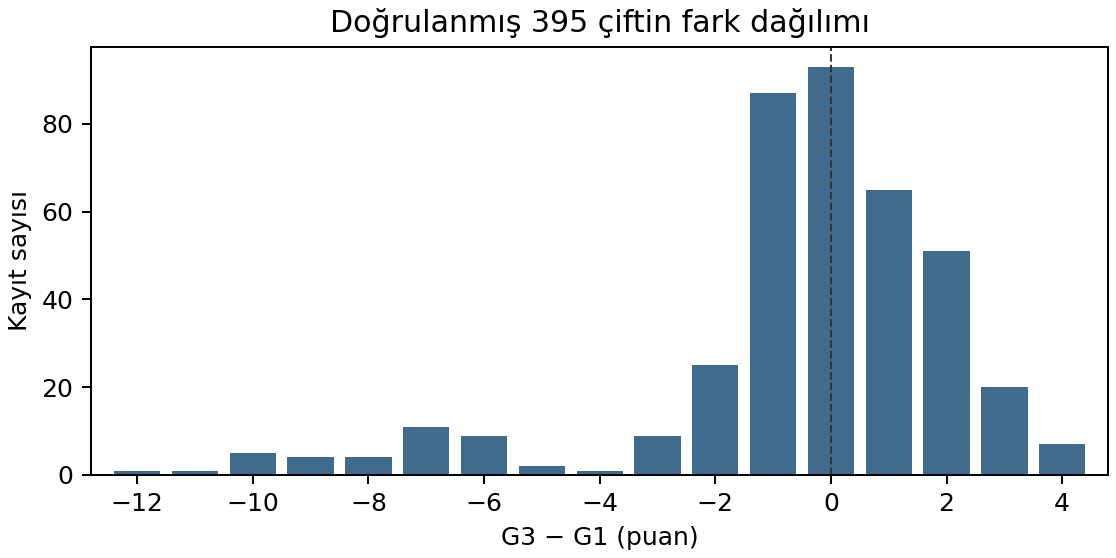
\includegraphics[width=\linewidth]{companion/vakalar/v3-eslesme/differences.png}
\caption{V3'te doğrulanmış G3--G1 farklarının sayımları. Sıfır G3
notları korunmuştur; yapay hatalı eşleşmeler grafiğe dahil değildir.}
\label{fig:v3-farklar}
\end{figure}

\textbf{Farkların anlamı.} Doğru eşleşmede 159 fark negatif, 93 fark
sıfır, 143 fark pozitiftir. Medyan 0; en küçük fark $-12$, en büyük
fark 4 puandır. Ortalama farkın negatif olması her öğrencinin notunun
düştüğü anlamına gelmez. Grafik, kimin öğretimden ne kadar yararlandığını
veya farklı öğrencilerin bağımsızlığını kanıtlamaz. Dönem notlarının
nasıl oluşturulduğu açıklanmadan farkı yalnız öğrenme kaybı diye
adlandırmayız.

\textbf{Ham çift ile özet girdi.} Küçük B14 paketindeki 24 çift,
ortalama fark $-3{,}2$ ve fark standart sapması 6 bilgisi başka bir
öğretim örneğidir; bu 395 kaydın özeti değildir. O üç özetten standart
hata ve test hesabı yapılabilir; hangi kişinin eksik eşinin bulunduğu,
anahtarların yinelenmesi veya fark grafiği geri kurulamaz. Aynı özeti
veren farklı ham veriler olabilir; 24 çifti bu veriden türetmeyiz.

\subsection{Görevler, kontrol yanıtları ve puanlama}
Her görevin iki bileşeni vardır. Bileşen başına doğru, gerekçeli yanıt
1 puan; eksik veya yanlış yanıt 0 puandır. Toplam 10 puan.

\begin{enumerate}
\item \textbf{Anahtar ve birim.} \texttt{id}'nin kökenini açıklayın;
ayrı sıralanmış iki tabloyu yeniden numaralandırmak yerine doğru
eşleşmeyi nasıl koruyacağınızı yazın.
\item \textbf{Yanlış eşleşmeyi yakalama.} Tablodaki iki ortalama
neden aynıdır? Buna rağmen ikinci satır neden geçerli değişim
analizi değildir?
\item \textbf{İki tür eksiklik.} Bir satırın yokluğu ile notun
boşluğu için anahtar eşleşmesi/tam çift sayısını ayrı yazın. Yinelenen
anahtarda neden otomatik olarak ilk kayıt alınmamalıdır?
\item \textbf{Dağılım ve yorum.} Negatif ortalamayı herkesin notunun
düşmesi şeklinde yorumlayan cümleyi sayımlarla düzeltin; ardından
bu farkın neden tek başına öğretimin nedensel etkisi olmadığını açıklayın.
\item \textbf{Özetin sınırı.} Küçük B14'ün 24 çiftlik özetinden
bir hesaplanabilir nicelik ve bir denetlenemeyecek kayıt özelliği
verin. Bu özeti mevcut 395 çiftle birleştirmemenizin nedenini belirtin.
\end{enumerate}

\textbf{Gerekçeli kontrol yanıtları.}
\begin{enumerate}
\item Yerel anahtar kaynak satırına bağlıdır; özgün kişi kimliği değildir
(1). Bölmeden önce korunur, kaynakla denetlenir ve tablolar bu sabit
anahtarla birleştirilir; yeniden sıra numarası üretilmez (1).
\item Her sütunun toplamı değişmediğinden ortalama fark korunur (1).
394 yanlış ortak nedeniyle farklar artık aynı öğrencinin iki notu
değildir; standart sapmanın da değişmesi hatayı görünür kılar (1).
\item Satır yoksa 394/394, yalnız not eksikse 395/394 bulunur (1).
Yinelenme kaynak kayıtlarına dönülerek çözülmelidir; ilk satırı seçmek
ölçüm veya anahtar hatasını gizleyebilir (1).
\item 159 negatif yanında 93 sıfır ve 143 pozitif fark bulunduğundan
``herkesin notu düştü'' yanlıştır (1). Eşdeğer ölçüm ve rastgele
müdahale ataması bu kayıtlardan doğrulanmaz; puan farkı tek başına
öğretim etkisi değildir (1).
\item Standart hata $6/\sqrt{24}$ hesaplanabilir, fakat ham
anahtar/eş eksikliği denetlenemez (1). Bunlar farklı öğretim örnekleridir;
24 çift bu 395 gözlemin alt grubu veya bağımsız tekrarı sayılamaz (1).
\end{enumerate}

\textbf{Kısa rapor örneği.} ``Kaynak satırıyla eşleştirilen sabit
yerel anahtarlar üzerinden 395 tam çift doğrulanmış; sıfır yıl sonu
notları korunmuştur. G3 eksi G1 ortalama farkı $-0{,}494$ puan,
medyanı 0'dır; 159 negatif, 93 sıfır ve 143 pozitif fark vardır.
Bu betimleme eşdeğer sınavlardan elde edilen öğrenme kaybı veya
bir öğretim müdahalesinin nedensel etkisi olarak sunulmamıştır.''

Python aktarımı ve ayrı anahtar sözlüğüyle hesap kontrol edilmiştir;
yeni R/SPSS çalıştırması veya bağımsız saha kimliği doğrulaması
yapılmamıştır. Kod, sözlük, hata denemeleri ve dosya özetleri
\nolinkurl{companion/vakalar/v3-eslesme/} klasöründedir.

\section{Bölüm özeti}

\begin{itemize}
  \item Test seçimi ölçümlerin bağımsız veya eşleştirilmiş oluşuna dayanır.
  \item Welch testi iki bağımsız ortalamayı eşit varyans zorunluluğu olmadan karşılaştırır.
  \item Eşleştirilmiş testin analiz birimi bireysel ölçüm değil, fark puanıdır.
  \item Pozitif eşleşme korelasyonu fark puanının standart hatasını azaltabilir.
  \item Eksik çiftler analiz örneklemini ve sonuçların temsilini etkileyebilir.
  \item Ortalama farkı güven aralığı, etki büyüklüğü ve tasarım sınırlarıyla raporlanmalıdır.
\end{itemize}

\section*{Alıştırmalar}

\begin{enumerate}
  \item Bağımsız ve eşleştirilmiş tasarıma birer eğitim araştırması örneği verin.
  \item Eşleştirilmiş testte neden fark puanlarının dağılımının incelendiğini açıklayın.
  \item Welch testinin klasik eşit varyanslı teste tercih edilme gerekçesini yazın.
  \item İki grubun eşit örneklem hacmine sahip olmasının neden eşleşme göstermediğini açıklayın.
  \item Grup 1 eksi grup 2 farkıyla grup 2 eksi grup 1 farkının güven aralıklarını karşılaştırın.
  \item $n_1=36$, $s_1=12$, $n_2=49$, $s_2=14$ için farkın standart hatasını hesaplayın.
  \item Ortalama farkı 5 ve standart hatası 2 ise Welch t değerini bulun.
  \item $n=16$, $\bar d=3$, $s_D=6$ için eşleştirilmiş t değerini hesaplayın.
  \item Ön test ve son test standart sapmaları 8, korelasyon 0,50 ise farkların standart sapmasını bulun.
  \item Korelasyon arttıkça eşleştirilmiş testin standart hatasının neden azalabileceğini açıklayın.
  \item Eşleştirilmiş analizde 40 katılımcıdan yalnız 34'ünün tam çifti varsa $n$ ve $sd$ değerlerini yazın.
  \item Welch testinde kesirli serbestlik derecesinin neden hata olmadığını açıklayın.
  \item Güven aralığı $[-1;9]$ olan 4 puanlık grup farkını yorumlayın.
  \item Anlamlı grup farkının neden rastgele atama olmadan nedensel etki göstermediğini açıklayın.
  \item Cohen $d$, Hedges $g$ ve $d_z$ değerlerinin tanımlarının neden raporda belirtilmesi gerektiğini tartışın.
  \item Eşleştirilmiş veriyi bağımsız testle analiz etmenin sonuçlarını standart hata bakımından açıklayın.
\end{enumerate}